\documentclass[12pt]{article}

\usepackage[utf8]{inputenc}
\usepackage[T1, T2A]{fontenc}
\usepackage[russian]{babel}

\usepackage{amsmath,amssymb}

\usepackage{float}
\usepackage{graphicx}
\graphicspath{ {./pic/} }

\title{Байесовская деконволюция для эксперимента СФЕРА-2}

\author{Игорь Вайман}

\date{\today}

\begin{document}
	\maketitle
	
	\section{Описание эксперимента}

	Эксперимент СФЕРА-2 основан на сборе и регистрации черенковского света ШАЛ, отражённого от <<экрана>> -- ровной заснеженной поверхности льда озера Байкал. Установка представляет собой сферическое зеркало и мозаику ФЭУ, установленную вблизи фокальной поверхности. Черенковский свет ШАЛ, рассеиваясь на снегу, проходит через диафрагму установки, отражается от зеркала, и попадает на фотокатод. При попадании фотона с длиной волны в области чувствительности фотокатода с него выбиваются $1 - 10$ (уточнить) вторичных электронов, которые проходят систему динодов с разностью потенциалов между каждой парой, создавая в результате избыточный на аноде. Этот заряд стекает с анода через цепь усиления, создавая в результате напряжение на входе АЦП. Это напряжение считывается электроникой, в результате и составляя (вместе с некоторой телеметрией) экспериментальные данные.
	
	Этот набор физических процессов мы описываем в следующих предположениях:
	
	\begin{enumerate}
		\item В системе нет электронных шумов -- единственным источником шума являются фоновые фотоны (от звёздного и зодиакального света, так как эксперимент проводится в ясные безлунные ночи). Фотоны шума попадают в установку аналогично <<сигнальным>> фотонам -- после рассеяния на поверхности. Их поток можно приблизительно оценить по каталогам светимости звёзд и из моделей зодиакального света. (Ссылка на работу Энтиной)
		\item Работу ФЭУ можно эффективно описать одной <<рандомизированной>> испульсной характеристикой (РИХ). Понятие и применение РИХ будет раскрыто далее, в общем виде это случайная функция времени, описывающая отклик системы на один фотон, падающий на фотокатод. Главный источник случайности в установке СФЕРА-2 -- неопределённость числа вторичных фотонов, вылетевших с фотокатода, приводящая к неопределённости амплитуды импульса тока. Стоит отметить, что случайный характер ИХ проявляется именно на границе между режимом счёта фотонов и режимом измерения потока, поскольку поток фотонов уже слишком велик, чтобы разрешать отдельные импульсы, но недостаточно -- чтобы случайные характеристики эффективно усреднялись. Мы также предполагаем, что случайность импульсной характеристики проявлялась независимо между отдельными фотонами и между разными ФЭУ.
		\item Используя экспериментальные данные (данные, записанные АЦП, постоянную компоненту анодного тока и абсолютную калибровку ФЭУ) мы можем восстановить показания анодного тока (ссылка на работу по электронике). Неопределённость, вносимая анодной цепью, усилителем и (главным образом) дискретизацией сигнала на входе АЦП, хорошо известна и учитывается во вторую очередь.
	\end{enumerate}

	\section{Постановка задачи}
	
	\subsection{Упрощённая модель}
	
	Рассмотрим $N$ последовательных равновеликих временных бинов. Для простоты будем считать единицей времени длительность одного бина. Тогда мы можем задать временные бины интервалами $[i-1, i]$, $i = 1 \ldots N$. Обратим внимание, что при такой нумерации бинов эффект от фотонов, попавших в $i$-тый временной бин проявляется впервые в момент времени $i$. Это приводит к симметричной нумерации бинов и временных отсчётов. Обозначим число фотонов в каждом бине как $n_i$, $i = 1, \ldots, N$.

	\begin{figure}[t!]
		\centering
		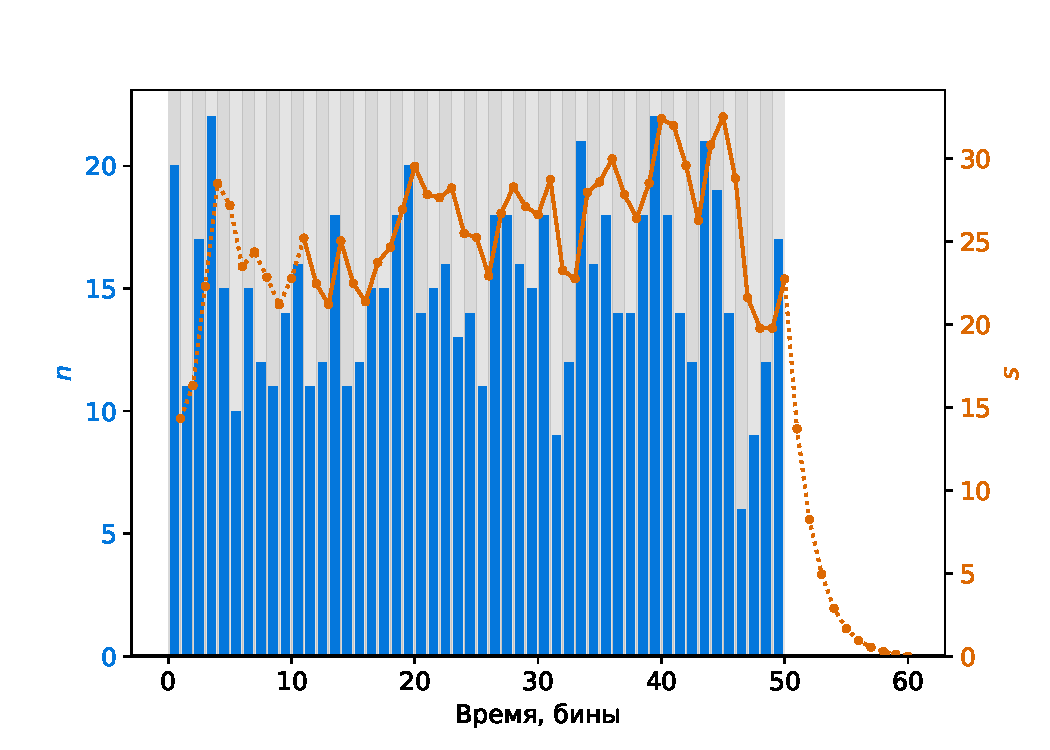
\includegraphics[width=\columnwidth]{problem-setup-example}
		\caption{Пример данных для задачи байесовской деконволюции. Здесь $N = 50$, количество фотонов в каждом бине определено из пуассоновского распределения с $\lambda = \mathbb{E}(n_i) = 15$; РИХ для простоты положена детерминистичной функцией $\exp(-t)$ с $L = 10$. Задача состоит в том, чтобы, зная значения выходного сигнала (оранжевый) и РИХ, оценить апостериорные распределения количества фотонов в каждом бине (синих столбцов).}
		\label{pic:problem-setup}
	\end{figure}

	Время прихода фотона внутри бина -- также случайная величина, обозначим её $t_{inbin}$. Она может быть, вообще говоря, распределена произвольным образом в интервале $[ 0, 1 ]$, однако мы в простейшем случае будем считать $t_{inbin} \sim U(0, 1)$. Это оправдано для независимых друг от друга фоновых фотонов, и может служить приближением для фотонов ШАЛ в случае, если дисперсия времён прихода фотонов внутри <<пакета>> сильно превышает длительность временного бина. По данным модельных ливней это не всегда так, поэтому влияние неравномерности распределения времён прихода фотонов будет исследовано отдельно.

	Предположим, что импульсная характеристика системы -- случайная функция $\tilde{h}(t)$, любая реализация которой удовлетворяет условиям: 
	\begin{enumerate}
		\item Каузальности, то есть $\forall t < 0 \; \; \tilde{h}(t) = 0$
		\item Конечности во времени, то есть $\exists \tilde{L}$ такое, что $\forall t > \tilde{L} \; \; \tilde{h}(t) = 0$.
	\end{enumerate}

	Заметим, что эффект от фотонов в $i$-том бине проявляется в отсчётах c $i$ по $i + \left \lfloor{\tilde{L}}\right \rfloor$, где $\left \lfloor{\tilde{L}}\right \rfloor$ -- целая часть или округление вниз $\tilde{L}$. Обозначим $L \equiv \left \lfloor{\tilde{L}}\right \rfloor$. Тогда полный сигнал от фотонов гарантированно содержится в отсчётах с $1$ по $N + L$.
	
	Будем считать, что АЦП записывает значения сигнала $S_j$ в точках $j = 1, \ldots, N + L$.
	
	Поставим задачу <<байесовской деконволюции>> следующим образом, используя байесовскую терминологию: зная рандомизированную импульсную характеристику системы и значения $S_j, \; j = 1, \ldots, N + L$, оценить апостериорные функции плотности вероятности для значений $n_i$, $i = 1, \ldots, N$. В качестве априорного распределения $n_i$ используется наивное неограниченное однородное распределение ($p_{n_i}(x) = Const \; \forall x \in [0, \infty)$).
	
	Заметим, что, в отличие от обычной деконволюции, мы не ставим задачу оценить исходный сигнал -- в данном случае представляющий собой сумму $\delta$-функций с соответствующими сдвигами -- но только его аггрегированную характеристику. Информация об отдельных фотонах не является необходимой для обработки экспериментальных событий, и её получение представляет собой, по-видимому, более трудную задачу.
	
	Легко заметить также, что в реальном эксперименте мы имеем дело с неограниченным во времени потоком фотонов, а не с изолированными $N$ бинами -- эффекты на краях области регистрации сигнала нужно будет учитывать отдельно.
	
	Иллюстрация постановки задачи приведена на рис. \ref{pic:problem-setup}.

	\subsection{Выходной сигнал как реализация случайного процесса}

	Очевидно, что $\{ S_j \}$ -- случайные величины, как в силу того, что РИХ в общем случае представляет собой случайную функцию, так и в силу принципиально случайного распределения фотонов внутри временного бина.
	
	Можно записать $S_j$ как сумму вкладов от фотонов разных бинов
	
	\begin{equation}
		S_j = \sum_{l=0}^{L} C(n_{j-l}, l)
	\end{equation}

	Здесь $C(n, l)$ -- случайная величина, описывающая вклад в сигнал на $j$-том временном отсчёте от $n$ фотонов в бине $j - l$, иначе говоря, вклад с \textit{задержкой} $l$ бинов. Из-за схемы индексации бинов и определения $L$ задержка изменяется в пределах от $0$ до $L$.
	
	Случайную величину $C(n, l)$, очевидно, можно выразить через РИХ. Проще всего сделать это через Монте-Карло-сэмплирование распределения. Получим с произвольной точностью эмпирическую функцию плотности распределения для величины $C(1, l)$. Для этого сгенерируем значения $t_i \sim t_{inbin};$ и функции $h_i(t) \sim \tilde{h}(t)$ для $i = 1 \ldots N_{sample}$. Выборка для $C(1, l)$ тогда будет состоять из значений $h_i(l + 1 - t_i)$. Выборка для $C(n, l)$ легко получить, проделав описанную процедуру $n$ раз и сложив все $n$ реализаций $N_{sample}$-мерных векторов выборок.
	
	\subsubsection{Средние значения}
	
	С вычислительной точки зрения нетрудно заранее вычислить для данной РИХ значения $C(1, l)$ для $l = 0 \ldots L$. Так как фотоны независимы друг от друга, то из этих эмпирических распределений оказывается возможно записать уравнения на средние значения величин $S_j$. А именно, обозначая $c_l \equiv C(1, l)$,
	
	\begin{equation}
		\hat{S}_j = \mathbb{E} \; S_j = \sum_{l=0}^{L} \mathbb{E} \; C(n_{j-l}, l) = \sum_{l=0}^{L} n_{j-l} \; \mathbb{E} \; C(1, l) = \sum_{l=0}^{L} n_{j-l} c_l
	\end{equation}

	Суммирование можно записать в матричном виде:
	
	\begin{equation}
		\begin{pmatrix} 
			c_0   &  0   &  0   &\dotsm&   0     \\
			c_1   & c_0  &  0   &\dotsm&  0     \\
			c_2   & c_1  & c_0  &      & \vdots \\
			c_3   & c_2  & c_1  &\ddots&  0     \\
     	    \vdots& c_3  & c_2  &\ddots&  c_0   \\
			c_L   &      & c_3  &\ddots&  c_1   \\
			0     & c_L  &      &\ddots&  c_2   \\
			\vdots&      & c_L  &      &  c_3   \\
			0     &\dotsm&  0   &\ddots& \vdots \\
			0     &\dotsm& 0    &   0  &  c_L   \\
		\end{pmatrix}
		\begin{pmatrix} 
			n_1 \\ n_2 \\ \vdots \\ n_N
		\end{pmatrix}
		=
		\begin{pmatrix} 
			\hat{S}_1 \\ \hat{S}_2 \\ \vdots \\
			\hat{S}_N \\
			\hat{S}_{N+1} \\ \vdots \\ \hat{S}_{N+L}
		\end{pmatrix}
	\end{equation}
	
\end{document}
